The successful ROP attack works very well, as shown by the device executing the injected code in Figure \ref{fig::ex}.  The stack before the exploit is shown in Figure \ref{fig::st1}, with the corrupted stack shown in Figure \ref{fig::st2}. The flash memory is shown in the following states: original, erased, written, and rewritten in Figures \ref{fig::fl0}, \ref{fig::fl1}, \ref{fig::fl2}, \ref{fig::fl3}. 
\begin{figure}[htbp]
	\centering
	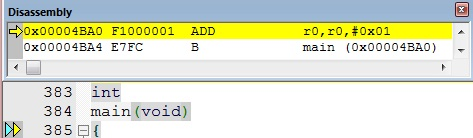
\includegraphics[scale=0.7]{ex2}
	\caption{The device executing the injected code. }\label{fig::ex}
\end{figure}


\begin{figure}[p]
	\centering
	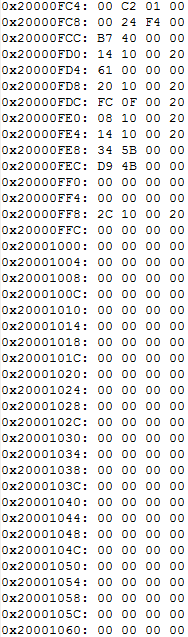
\includegraphics[\width=0.5\textwidth]{StackBefore1}
	\caption{The stack prior to any tampering. }\label{fig::st1}
\end{figure}
\begin{figure}[p]
	\centering
	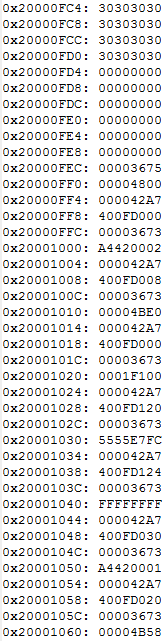
\includegraphics[\width=0.5 \textwidth]{stackAfter}
	\caption{The stack after corruption. }\label{fig::st2}
\end{figure}

\begin{figure}[p]
	\centering
	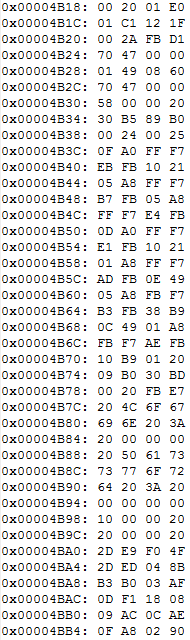
\includegraphics[\width=1in]{FlashBefore.PNG}
	\caption{The flash memory at main prior to any tampering. }\label{fig::fl0}
\end{figure}
\begin{figure}[p]
	\centering
	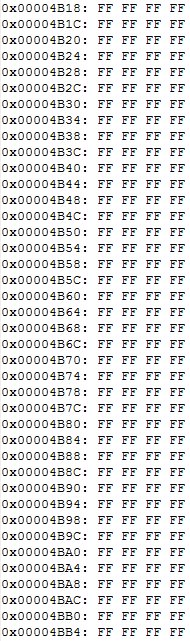
\includegraphics[\width=0.5\textwidth]{FlashAfterErase}
	\caption{The flash memory after the erase of main(). }\label{fig::fl1}
\end{figure}

\begin{figure}[p]
	\centering
	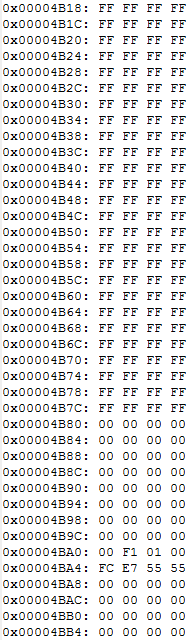
\includegraphics[\width=0.5\textwidth]{FlashAfterWrite1}
	\caption{The flash memory after the write to main(). }\label{fig::fl2}
\end{figure}

\begin{figure}[p]
	\centering
	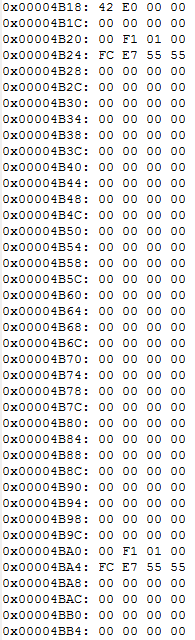
\includegraphics[\width=0.5\textwidth]{FlashAfterWrite2}
	\caption{The flash memory after the write to the scatter function. }\label{fig::fl3}
\end{figure}
